\documentclass[a4paper,12pt]{article}
\usepackage[a4paper, top=2cm, bottom=2cm]{geometry}
\usepackage{amsmath} % Để sử dụng môi trường toán học và lệnh aligned
\usepackage{tkz-tab}
\usepackage[vietnamese]{babel}
\usepackage[utf8]{vietnam}
\usepackage{xcolor}
\usepackage{listings}
\usepackage{enumitem}
\usepackage{hyperref}
\usepackage{amsmath}
\usepackage{amssymb}
\usepackage{indentfirst}
\usepackage{float}
% Cấu hình lại hyperlink
\hypersetup{
    colorlinks=true,
    linkcolor=black, % Màu đen cho các liên kết trong mục lục
    filecolor=black,
    urlcolor=black,
    citecolor=black
}
\usepackage{caption}
% \captionsetup[figure]{labelformat=empty}
\urlstyle{same}
\definecolor{codegray}{rgb}{0.5,0.5,0.5}
\definecolor{codegreen}{rgb}{0,0.6,0}
\definecolor{codepurple}{rgb}{0.58,0,0.82}
\definecolor{backcolour}{rgb}{0.95,0.95,0.92}
\definecolor{codecomment}{rgb}{0,0.5,0.1}

\setlength{\parskip}{0.5em}
\renewcommand{\thesection}{\arabic{section}.}
\renewcommand{\thesubsection}{\thesection\arabic{subsection}.}
\renewcommand{\thesubsubsection}{\thesubsection\arabic{subsubsection}.}

\lstdefinestyle{mystyle}{
    backgroundcolor=\color{backcolour},
    commentstyle=\color{codecomment},
    keywordstyle=\color{magenta},
    numberstyle=\tiny\color{codegray},
    stringstyle=\color{codepurple},
    basicstyle=\footnotesize,
    breakatwhitespace=false,
    breaklines=true,
    captionpos=b,
    keepspaces=true,
    numbersep=5pt,
    showspaces=false,
    showstringspaces=false,
    showtabs=false,
    tabsize=2,
    language={[5.3]Lua}
}

\lstset{style=mystyle}

\begin{document}


\begin{titlepage}

\begin{center}

\textbf{TRƯỜNG ĐẠI HỌC CÔNG NGHỆ THÔNG TIN}

\textbf{KHOA KHOA HỌC MÁY TÍNH}

\vspace{1cm}

\textbf{BÁO CÁO ĐỒ ÁN CUỐI KÌ CS431}

\vspace{1cm}

\textbf{VanillaNet - Sức mạnh của Tối giản trong Học Sâu}

\vspace{1cm}
\includegraphics[width=5 cm]{logo.png}
\vspace{1cm}

\textbf{GV hướng dẫn: Nguyễn Vĩnh Tiệp}

\vspace{1cm}

\textbf{Nhóm 7:}

\vspace{0.5cm}

\begin{tabular}{p{5cm}p{5cm}}
\hline
\textbf{Họ và tên} & \textbf{MSSV} \\
\hline
Huỳnh Anh Dũng & 22520278\\
\hline
Hà Huy Hoàng & 22520460 \\
\hline
Nguyễn Duy Hoàng & 22520467\\
\hline
Lê Phước Trung & 20522069 \\
\hline
\end{tabular}

\vspace{1cm}

\textbf{TP.HCM, ngày 9 tháng 1 năm 2025}

\newpage
\tableofcontents
\end{center}

\end{titlepage}


\newpage
\section{Giới thiệu}
Triết lý nền tảng của các mô hình hiện nay là `càng nhiều càng khác biệt' (`more is different'), điều này được chứng minh bằng các thành công vang dội trong lĩnh vực thị giác máy tính và xử lý ngôn ngữ tự nhiên. Một bước đột phá đáng chú ý trong các lĩnh vực này là sự phát triển của AlexNet \cite{NIPS2012_c399862d}, gồm 12 tầng và đạt hiệu suất hàng đầu trên chuẩn nhận dạng hình ảnh quy mô lớn. Xây dựng trên thành công này, ResNet \cite{he2015deepresiduallearningimage} giới thiệu các ánh xạ đồng nhất thông qua skip connections, cho phép đào tạo các mạng nơ-ron sâu với hiệu suất cao trên nhiều ứng dụng thị giác máy tính, như phân loại hình ảnh, phát hiện đối tượng và phân đoạn ngữ nghĩa. Việc kết hợp các module được thiết kế bởi con người trong những mô hình này, cũng như sự gia tăng liên tục về độ phức tạp của mạng không thể phủ nhận rằng đã nâng cao hiệu suất. 

Tuy nhiên, các thách thức về việc tối ưu hóa và sự phức tạp vốn có của các mô hình transformer kêu gọi một sự chuyển đổi mô hình hướng tới sự đơn giản. Trong báo cáo này, chúng em sẽ giới thiệu về \textbf{VanillaNet}, một cấu trúc mạng neural network mang tính tinh tế trong thiết kế. Bằng cách tránh độ sâu cao, các lối tắt, và các thao tác phức tạp như self-attention, VanillaNet vô cùng ngắn gọn nhưng lại đáng kinh ngạc về sức mạnh. Mỗi tầng được chế tác một cách cẩn thận để trở nên gọn gàng và thẳng thắn, với các hàm kích hoạt phi tuyến được loại bỏ sau quá trình huấn luyện để phục hồi kiến trúc ban đầu. VanillaNet vượt qua những thách thức của sự phức tạp vốn có, khiến nó trở nên lý tưởng cho các môi trường hạn chế tài nguyên.

\section{Kiến trúc Vanilla Neural}
Với sự phát triển của chip AI, vấn đề bottleneck về tốc độ suy luận của mạng neural không phải là FLOPs hay các tham số mà là do độ sâu và tính phức tạp trong thiết kế 
đã cản trở tốc độ. Để giải quyết vấn đề này, các tác giả của bài báo mà chúng em đang nghiên đã đề xuất VanillaNet \cite{chen2023vanillanetpowerminimalismdeep}, có cấu trúc được thể hiện trong Hình 1. VanillaNet tuân theo thiết kế phổ biến của mạng neural với stem block, main body và lớp fully connected. Khác với các mạng sâu hiện có, VanillaNet chỉ sử dụng một lớp trong mỗi giai đoạn để thiết lập một mạng cực kỳ đơn giản với số lượng lớp ít nhất có thể.
\begin{figure}[h!]
\centering
\includegraphics[width=15cm]{vanillanet-6-structure.png}
\caption{Kiến trúc của mô hình VanillaNet-6}
\end{figure}
\newpage
Chúng em sẽ làm rõ kiến trúc của VanillaNet trong phần này, lấy ví dụ là VanillaNet 6 như trong Hình 1. Đối với lớp stem, VanillaNet sẽ sử dụng một lớp tích chập 4x4x3x$\mathcal{C}$ với stride là 4 để chuyển đổi ảnh đầu vào 3 kênh màu (RGB) thành C kênh đặc trưng. Tại giai đoạn 1,2 và 3, một lớp maxpooling(stride=2) được sử dụng để giảm kích thước và feature map 2 lần đồng thời nó cũng tăng số lượng kênh lên gấp đôi sau mỗi giai đoạn. Ở giai đoạn 4, mạng không tăng số lượng kênh nữa mà thay vào đó là một lớp avarage pooling dùng để tóm tắt các thông tin đặc trưng đã học. Lớp cuối cùng là một lớp fully connected tương đương với output của mô hình phân loại này (lớp cuối cùng có kích thước 1x1x1000 vì mô hình này được huấn luyện trên bộ ImageNet-1K \cite{imagenet}). Kích thước nhân của mỗi lớp tích chập là 1x1 bởi vì VanillaNet hướng tới việc sử dụng tối thiểu chi phí cho mỗi lần tính toán mỗi lớp mà vẫn giữ thông tin của các feature map. Hàm kích hoạt được áp dụng sau mỗi lớp tích chập 1x1. Để đơn giản cho quá trình trainning của mạng, batch normalization cũng được thêm vào sau mỗi lớp. Cần lưu ý rằng VanillaNet không có skip connections, vì theo như trong bài báo có đề cập là các tác giả thấy việc thêm skip connections cho thấy ít cải thiện hiệu suất. Theo nhóm bọn em, việc cải thiện hiệu suât bằng cách thêm skip connections không có hiệu quả cao bởi vì mạng như VanillaNet thường không có số lượng lớp rất sâu (như ResNet hoặc DenseNet). Do đó, các vấn đề như mất mát thông tin hoặc vanishing gradient ít nghiêm trọng hơn.
Khi mạng không quá sâu, dòng chảy thông tin và gradient có thể được bảo toàn đủ tốt mà không cần skip connections. Điều này cũng mang lại một lợi ích khác là kiến trúc được đề xuất cực kỳ dễ thực hiện vì không có nhánh và các blocks bổ sung như khối squeeze và excitation. 

Bởi vì kiến trúc của VanillaNet đơn giản và tương đối nông nên tính phi tuyến tính yếu của nó gây ra hạn chế hiệu suất, Do đó, trong bài báo cũng đã đề xuất một loạt các kỹ thuật để giải quyết vấn đề này.

\section{Huấn luyện mạng VanillaNet}
Thông thường trong học sâu để nâng cao hiệu suất của các mô hình bằng cách giới thiệu khả năng mạnh mẽ hơn trong giai đoạn đào tạo \cite{chen2021universaladderneuralnetworks}. Để đạt được mục tiêu này, bài báo đã đề xuất sử dụng kỹ thuật đào tạo sâu để nâng cao khả năng trong quá trình đào tạo trong VanillaNet được đề xuất, vì mạng sâu có tính phi tuyến tính mạnh hơn mạng nông.
\subsection{Chiến lược đào tạo sâu}
Ý tưởng chính của chiến lược đào tạo sâu là huấn luyện hai lớp tích chập với một hàm kích hoạt thay vì một lớp tích chập ở giai đoạn ban đầu của quá trình huấn luyện. Hàm kích hoạt được giảm dần dần thành một ánh xạ đồng nhất với số chu kỳ huấn luyện gia tăng. Ở cuối giai đoạn huấn luyện, hai lớp tích chập có thể dễ dàng kết hợp lại thành một lớp tích chập để giảm thời gian suy luận. Dạng ý tưởng này đã được sử dụng rộng rãi trong CNN \cite{ding2021diversebranchblockbuilding, ding2021repvggmakingvggstyleconvnets, ding2022scalingkernels31x31revisiting, ding2019acnetstrengtheningkernelskeletons}. Sau đây, chúng em sẽ mô tả cách tiến hành kỹ thuật một cách chi tiết.

Cho hàm kích hoạt $A(x)$ (các hàm thường sử dụng như ReLU và Tanh), chúng em kết hợp với một ánh xạ đồng nhất, có thể viết dưới dạng toán học như sau:
\begin{center}
    $A'(x) = (1-\lambda)A(x) + \lambda x \hspace*{5mm} \textbf{(1)}$
\end{center}
trong đó $\lambda$ là một siêu tham số để cân bằng tính phi tuyến tính của việc hàm kích hoạt $A'(x)$. 

Ký hiệu số chu kỳ hiện tại và tổng số chu kỳ của việc huấn luyện sâu lần lượt là $e$ và $E$. Đặt $\lambda = \frac{e}{E}$. Vì vậy, khi bắt đầu giai đoạn huấn luyện $(e=0)$, $A'(x) = A(x)$, có nghĩa rằng mạng sẽ có tính phi tuyến tính mạnh. Khi quá tình huấn luyện hội tụ, chúng ta sẽ có $A'(x) = x$, có nghĩa là giữa hai lớp tích chập không có bất cứ hàm kích hoạt nào. Sau đây, chúng em sẽ làm rõ cách nào có thể kết hợp hai lớp tích chập này.

Đầu tiên, chúng tôi chuyển đổi tất cả lớp batch normalization và lớp tích chập trước đó của nó thành một tích chập duy nhất. Chúng ta ký hiệu $W \in \mathbb{R}^{C_{out}\times(C_{in}\times k \times k)}$, $B \in \mathbb{R}^{C_{out}}$ như là ma trận trọng số và ma trận sai số của nhân tích chập với $C_{in}$ kênh đầu vào, $C_{out}$ kênh đầu ra và kích thước nhân $k$. Các giá trị tỷ lệ, dịch chuyển, trung bình và phương sai trong batch normalization được biểu diễn lần lượt là $\gamma, \beta, \mu, \sigma \in R^{C_{out}}$. Các ma trận trọng số và bias được hợp nhất như sau:
\begin{center}
    $W'_i = \frac{\gamma_i}{\sigma_i}W_i, \hspace*{2mm} B'_i = \frac{(B_i - \mu_i)\gamma_i}{\sigma_i} + \beta_i  \hspace*{5mm} \textbf{(2)}$
\end{center}
trong đó $i \in \{ 1, 2, 3, ..., C_{out} \} $ ký hiệu cho giá trị trong kênh đầu ra thứ i.

Sau khi kết hợp lớp tích chập với batch normalization, chúng ta sẽ bắt đầu kết hợp hai lớp tích chập $1\times 1$. Gọi $x \in \mathbb{R}^{C_{in}\times H \times W}$ và $y \in \mathbb{R}^{C_{out}\times H' \times W'}$ là các đặc trưng đầu vào và đặc trưng đầu ra, lớp tích chập có thể biểu diễn như:
\begin{center}
    $y = W * x = W \cdot \text{im2col}(x) = W \cdot X \hspace*{5mm} \textbf{(3)}$
\end{center}
trong đó * là phép tích chập, $\cdot$ là phép nhân ma trận và $X \in \mathbb{R}^{(C_{in}\times 1 \times 1) \times (H' \times W')}$ xuất phát từ im2col \cite{qochuk_im2col} để chuyển đổi từ đầu vào thành một ma trận tương ứng với hình dạng của nhân. May mắn thay, đối với lớp convolution $1\times 1$, các tác giả của bài báo thấy rằng im2col trở thành một phép reshape đơn giản bởi vì không cần trượt các hạt nhân có sự chồng chéo. Do đó, ký hiệu ma trận trọng số của hai lớp tích chập là $W^1$ và $W^2$, hai lớp tích chập không có hàm kích hoạt có thể viết dưới dạng biểu thức sau:
\begin{center}
    $y = W^1 * (W^2*x) = W^1\cdot W^2 \cdot \text{im2col}(x) = (W^1 \cdot W^2) * X \hspace*{5mm} \textbf{(4)}$
\end{center}
Do đó, lớp convolution $1\times 1$ có thể hợp nhất với nhau mà không giảm tốc độ suy luận.

\subsection{Chồng chất hàm kích hoạt}
Đã có những đề xuất về hàm kích hoạt cho mạng bao gồm hàm được sử dụng rộng rãi như Rectified Linear Unit (ReLU) và các biến thể của nó (PReLU \cite{he2015delvingdeeprectifierssurpassing}, GeLU \cite{hendrycks2023gaussianerrorlinearunits} và Swish \cite{ramachandran2017searchingactivationfunctions}). Chúng chủ yếu tập trung vào nâng cao hiệu suất của mạng sâu vào phức tạp bằng cách sử dụng các hàm kích hoạt khác nhau. Tuy nhiên, như đã được chứng minh bởi các công trình đi trước \cite{mhaskar2016deepvsshallownetworks, eldan2016powerdepthfeedforwardneural, telgarsky2016benefitsdepthneuralnetworks}, giới hạn về sức mạnh của các mạng nông và cơ bản thường là do tính phi tuyến tính yếu của chúng, đây là điểm khác biệt so với các mạng sâu và phức tạp và do đó chưa được nghiên cứu đầy đủ.

Thực tế, có hai cách để cải thiện tính phi tuyến của mạng neural: xếp chồng các lớp kích hoạt phi tuyến hoặc tăng tính phi tuyến của từng lớp kích hoạt. Tuy nhiên, xu hướng của các mạng hiện tại thường chọn cách thứ nhất, điều này dẫn đến độ trễ cao khi khả năng tính toán song song vượt quá giới hạn.

Một ý tưởng trực quan để cải thiện tính phi tuyến của lớp kích hoạt là xếp chồng. Việc xếp chồng tuần tự các hàm kích hoạt là ý tưởng cốt lõi của các mạng neural sâu. Ngược lại, bài báo đã chuyển sang xếp chồng đồng thời các hàm kích hoạt. Ký hiệu một hàm kích hoạt đơn lẻ cho đầu vào $x$ trong mạng nơron là $A(x)$, có thể là các hàm phổ biến như ReLU và Tanh. Việc xếp chồng đồng thời $A(x)$ có thể được biểu diễn dưới dạng:
\begin{center}
    $A_s(x)=\displaystyle\sum^n_{i=1}a_iA(x+b_i) \hspace*{5mm} \textbf{(5)} \label{eq:activation}$
\end{center}
trong đó n là số lượng các hàm kích hoạt được xếp chồng và $a_i$, $b_i$ lần lượt là hệ số tỷ lệ và độ lệch của từng hàm kích hoạt để tránh việc cộng dồn đơn giản. Tính phi tuyến của hàm kích hoạt có thể được cải thiện đáng kể bằng cách xếp chồng đồng thời. Phương trình \textbf{\hyperref[eq:activation]{5}} có thể được xem như một chuỗi trong toán học, đó là phép toán cộng nhiều đại lượng lại với nhau.

Để làm phong phú thêm khả năng xấp xỉ của chuỗi, VanillaNet cho phép hàm dựa trên chuỗi này học thông tin toàn cục bằng cách thay đổi các đầu vào từ các lân cận của chúng, điều này tương tự như BNET \cite{xu2020batchnormalizationenhancedlinear}. Cụ thể, với một đặc trưng đầu vào \( x \in \mathbb{R}^{H \times W \times C} \), trong đó \( H, W \) và \( C \) lần lượt là chiều rộng, chiều cao và số lượng kênh của nó, hàm kích hoạt được biểu diễn như sau:
\begin{center}
$A_s(x_h,w,c) = \displaystyle\sum_{i,j \in {-n,n}}a_{i,j,c}A(x_{i+h, j+w, c} + b_c) \hspace*{5mm} \textbf{(6)}$
\end{center}
trong đó $h \in \{1, 2,..., H\}$ , $w \in \{1,2,...,W\}$ và $c \in \{1,2,...,C\}$. Dễ thấy rằng khi n = 0,  hàm kích hoạt dựa trên chuỗi $A_s(x)$ suy giảm thành hàm kích hoạt thông thường $A(x)$, điều này có nghĩa rằng phương pháp đề xuất có thể được xem như một sự mở rộng tổng quát của các hàm kích hoạt hiện có. VanillaNet sử dụng ReLU làm hàm kích hoạt cơ bản để xây dựng chuỗi này, vì nó hiệu quả trong việc suy luận trên GPU.

Chúng tôi phân tích thêm độ phức tạp tính toán của hàm kích hoạt được đề xuất so với lớp tích chập tương ứng của nó. Đối với một lớp tích chập với kích thước kernel \( K \), số kênh đầu vào \( C_{in} \) và số kênh đầu ra \( C_{out} \), độ phức tạp tính toán là:
\begin{center}
    $\mathcal{O}(CONV) = H \times W \times C_{\text{in}} \times C_{\text{out}} \times k^2 \hspace*{5mm} \textbf{(7)}$
\end{center}
trong khi đó độ phức tạp tính toán của lớp chuỗi kích hoạt là:
\begin{center}
    $\mathcal{O}(SA) = H \times W \times C_{\text{in}} \times n^2 \hspace*{5mm} \textbf{(8)}$
\end{center}
Do đó, ta có:
\begin{center}
    $\displaystyle\frac{\mathcal{O}(CONV)}{\mathcal{O}(SA)} = \frac{H\times W \times C_{\text{in}} \times C_{\text{out}} \times k^2}{H \times W \times C_{\text{in}} \times n^2} = \frac{C_{\text{out}}\times k^2}{n^2} \hspace*{5mm} \textbf{(9)}$
\end{center}
Lấy giai đoạn 3 trong VanillaNet-6 làm ví dụ,trong đó $k = 1$ (như đã nói ở \hyperref[section]{phần 2}), $C_{\text{out}} = 4096$ và n = 3 (giá trị mặc định trong code của bài báo \cite{chen2023vanillanetpowerminimalismdeep}), tỷ lệ vào khoảng 455. Kết luận, chi phí tính toán của hàm kích hoạt được đề xuất vẫn thấp hơn nhiều so với các lớp tích chập. Phân tích chi tiết hơn về độ phức tạp thực nghiệm sẽ được trình bày trong phần sau.       

\section{Thực nghiệm}
\subsection{Bộ dữ liệu}
Để tiến hành thực nghiệm hiệu năng mô hình VanillaNet, nhóm nghiên cứu quyết định sử dụng bộ dữ liệu ``Ships in Satellite Imagery'' \cite{robert_hammell_2018} của tác giả Rhammell đăng tải trên Kaggle.

Hình ảnh từ vệ tinh cung cấp thấu quan đến nhiều lĩnh vực trong cuộc sống. Nhưng với sự phát triển đầy bùng nổ của ngành công nghiệp hàng không vũ trụ, việc lượng dữ liệu đổ dồn vượt mức xử lý thủ công của con người là không thể tránh khỏi. Mục tiêu của bộ dữ liệu đề ra hướng đến việc giải quyết bài toán hóc búa trong việc phát hiện vị trí tàu thủy từ vệ tinh. Việc tự động hóa bài toán nêu trên được cho rằng sẽ thúc đẩy sự phát triển của bộ máy quản lý chuỗi cung ứng, cụ thể hơn, trong lĩnh vực xuất nhập cảnh hải cảng.

\subsubsection{Nội dung}
Hình ảnh trong bộ dữ liệu được trích xuất từ bộ ảnh chụp của dịch vụ vệ tinh Planet, trong phạm vi vùng vịnh San Francisco và San Pedro bang California, bao gồm 4000 tấm ảnh có kích thước 80x80, lưu ở định dạng RGB. Mỗi ảnh đều mang nhãn phân loại bản thân ảnh là \textbf{``ship''} hoặc \textbf{``no-ship''}.

Một thư mục nén (.zip) được cung cấp, chứa toàn bộ tập dữ liệu dưới dạng hình ảnh .png. Tên tệp của từng hình ảnh tuân theo định dạng sau: 

\{label\} \_ \{scene id\} \_ \{longitude\} \_ \{latitude\}.png

\noindent Chi tiết:
\begin{itemize}
    \item label: Giá trị 1 hoặc 0, lần lượt đại diện cho lớp ``ship'' (tàu) và lớp ``no-ship'' (không phải tàu).
    \item scene id: Mã định danh duy nhất của cảnh trực quan PlanetScope mà hình ảnh được trích xuất. Mã này có thể được sử dụng với Planet API để tìm kiếm và tải xuống toàn bộ cảnh.
    \item longitude\_latitude: Tọa độ kinh độ và vĩ độ của điểm trung tâm hình ảnh, với giá trị được phân tách bằng dấu gạch dưới (\_).
\end{itemize}
\newpage
Ngoài ra, còn có một file JSON (file này nhóm không sử dụng trong quá trình thực nghiệm) chứa:
\begin{itemize}
    \item data: Dữ liệu pixel của từng ảnh.
    \begin{itemize}
        \item  6400 phần tử đầu tiên: Giá trị kênh màu đỏ (red).
        \item 6400 phần tử tiếp theo: Giá trị kênh màu xanh lá cây (green).
        \item 6400 phần tử cuối cùng: Giá trị kênh màu xanh dương (blue).
    \end{itemize}
    \item label: Nhãn của hình ảnh (1 hoặc 0).
    \item scene\_ids: Danh sách mã định danh cảnh tương ứng.
    \item locations: Tọa độ tương ứng.
\end{itemize}
\subsubsection{Nhãn phân loại}
Lớp ``ship'' (tàu) bao gồm 1000 hình ảnh. Các hình ảnh trong lớp này được căn giữa vào thân của một con tàu duy nhất. Các hình ảnh bao gồm tàu có nhiều kích thước, hướng và điều kiện khí quyển khác nhau.
\begin{figure}[H]
\centering
\includegraphics[width=15cm]{ship_image.png}
\caption{Một số ảnh trong bộ gán nhãn ``ship''}
\end{figure}

Lớp ``no-ship'' (không phải tàu) bao gồm 3000 hình ảnh. Các hình ảnh trong lớp này được chia thành ba nhóm:
\begin{itemize}
    \item Một phần ba đầu tiên: Là tập hợp ngẫu nhiên các đặc điểm địa hình khác nhau - nước, thảm thực vật, đất trống, tòa nhà, v.v. - không bao gồm bất kỳ phần nào của một con tàu.
    \item Một phần ba tiếp theo: Là các "phần của tàu" (partial ships) chỉ chứa một phần của con tàu, nhưng không đủ để đáp ứng định nghĩa đầy đủ của lớp "có tàu".
    \item Một phần ba cuối cùng: Là các hình ảnh từng bị dán nhãn sai bởi các mô hình học máy, thường do các điểm ảnh sáng hoặc các đặc điểm đường thẳng nổi bật.
\end{itemize} 
Các ví dụ về hình ảnh từ lớp này được hiển thị dưới đây.
\begin{figure}[H]
\centering
\includegraphics[width=15cm]{no-ship_image.png}
\caption{Một số hình ảnh của nhãn ``no-ship''}
\end{figure}
\subsubsection{Cảnh quan}
Tám hình ảnh toàn cảnh đầy đủ được bao gồm trong thư mục scenes. Các cảnh này có thể được sử dụng để trực quan hóa hiệu suất của các mô hình phân loại đã được huấn luyện trên tập dữ liệu.
\begin{figure}[H]
\centering
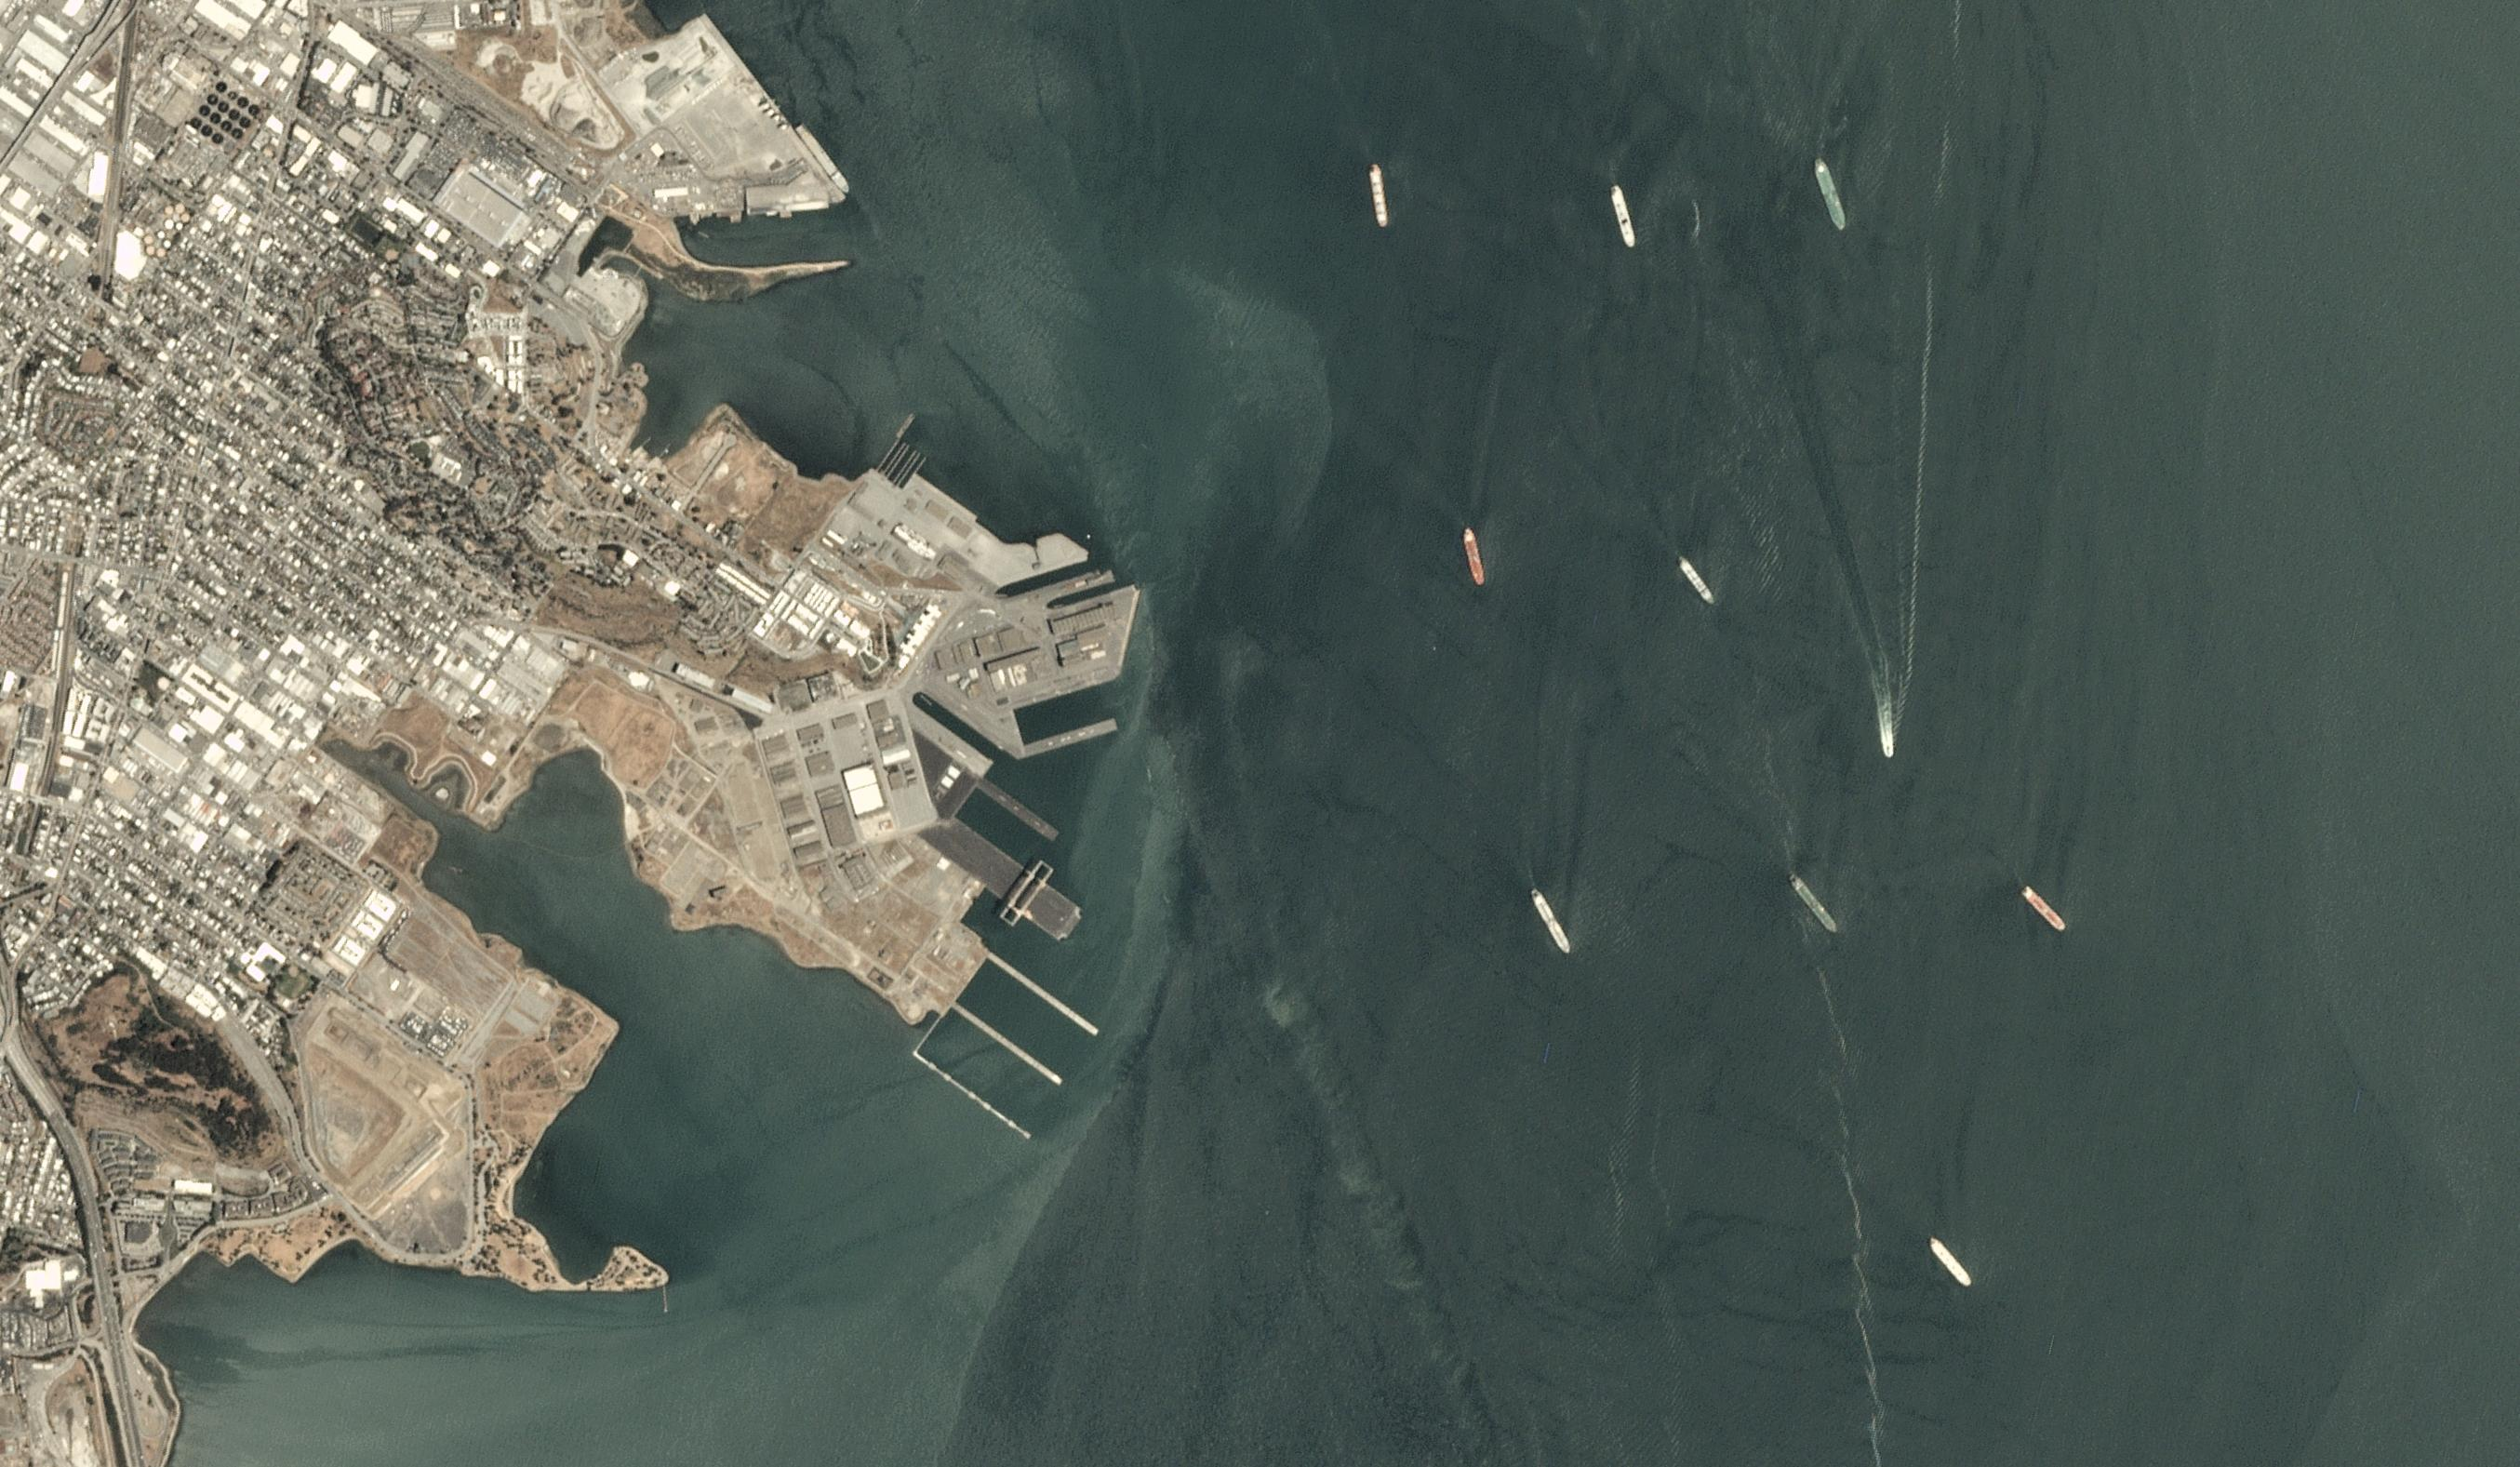
\includegraphics[width=15cm]{scene.png}
\caption{Một ảnh toàn cục trong bộ dữ liệu}
\end{figure}

\subsubsection{Tăng cường dữ liệu}
Nhận thấy số lượng ảnh không thực sự nhiều và đa dạng để các mô hình tiền huấn luyện có thể biểu diễn được hết khả năng, cũng như xét về tỉ lệ lệch lớp giữa các nhãn ``no-ship'' và ``ship'' khá lớn, cụ thể là 3:1 lần lượt theo thứ tự đã nêu, nhóm đã áp dụng một số biện pháp tăng cường dữ liệu tuy đơn giản nhưng đủ để tăng thêm tính đa dạng cũng như tạo điều kiện cho mô hình tiếp xúc với nhiều loại phân bố nhiễu khác nhau của cùng một khuôn mẫu, từ đó tăng cường tính phổ quát hơn cho mô hình.

Các biện pháp tăng cường nhóm sử dụng bao gồm:

\begin{itemize}
    \item Horizontal Flip: Lật ảnh theo phương ngang.
    \item Vertical Flip: Lật ảnh theo phương đứng.
    \item Shit Scale Rotate: Xê dịch, biến đổi kích cỡ và xoay ảnh.
    \item Random Brightness Contrast: Thay đổi ngẫu nhiên độ sáng và độ tương phản ảnh.
    \item Gaussian Blur: Làm mở Gaussian.
    \item Gauss Noise: Tạo nhiễu theo phân phối Gaussian.
\end{itemize}

Các biện pháp tăng cường đều được nhóm áp dụng theo tỉ xuất xảy ra ngẫu nhiên 50\%, bộ ảnh sau khi tăng cường được nhóm lưu vào ổ cứng cho mục đích tái sử dụng.

\subsection{Bài toán thực nghiệm}
Nhằm thực nghiệm khả năng trích xuất đặc trưng của mô hình, nhóm quyết định giải bài toán phát hiện vật thể trên bộ dữ liệu vừa nêu.

Bài toán trên được nhóm cài đặt qua hai bài toán con: phân loại và gán nhãn cho sliding window trong cảnh quan.

\subsection{Phương pháp}
Để thực hiện bài toán phân loại tàu thủy và bối cảnh, nhóm cần xây dựng được một mô hình học sâu phù hợp có số lớp đầu ra là hai lớp. Ý tưởng chính vẫn là dựa trên mô hình VanillaNet để cấu nên một mô hình mới sao cho phù hợp với yêu cầu. Nhận thấy VanillaNet, với số lớp đầu ra 1000, không thực sự thỏa mãn được yêu cầu bài toán, nhóm quyết định thay lớp fully-connected đầu cuối của mô hình ban đầu thành lớp có chức năng tương tự nhưng cho đầu ra phân loại hai lớp.

\subsubsection{Thay lớp đầu cuối}
Nhờ tính chất được phát triển với Pytorch, một thư viện hỗ trợ \emph{dynamic computing graph} (tạm dịch: đồ thị tính toán động), nhóm có thể dễ dàng xem cấu trúc của mô hình trên thực tế một cách đơn giản, chỉ với việc \emph{print} mô hình ra màn hình hiển thị trong môi trường phát triển,

\begin{figure}[H]
    \centering
    \includegraphics[width=\linewidth]{vanillanet-ondev.png}
    \caption{Sơ bộ về thuộc tính lớp VanillaNet trong Pytorch}
\end{figure}

\noindent so với mô hình nhóm thực hiện thay đổi.

\begin{figure}[H]
    \centering
    \includegraphics[width=\linewidth]{vanillanet-customized-ondev.png}
    \caption{Thuộc tính lớp VanillaNet sau khi thay lớp}
\end{figure}

Nhờ việc Pytorch xem các modules xuất hiện trong mô hình như thuộc tính của lớp mô hình đó, nhóm dễ dàng thực hiện việc loại bỏ và thay lớp bằng các lệnh \verb|delattr| và lệnh gán cho thuộc tính \verb|cls| của mô hình một lớp \verb|Linear| mới có số đặc trưng đầu ra là hai.

Cài đặt ban đầu của VanillaNet sử dụng lớp tích chập kích thước nhân 1x1 để thay thế cho lớp fully-connected, nhóm nhận thấy rằng việc này không thực sự cần thiết, đặc biệt khi phương pháp huấn luyện sâu không được áp dụng trong thực nghiệm, nhóm đề xuất việc tái cấu trúc mô hình với lớp fully-connected đồng thời định nghĩa luồng dữ liệu \verb|forward| mới bên trong của mô hình sao cho thỏa mãn cả cấu trúc xây dựng, cả đồ thị tính toán ban đầu.

\subsubsection{Huấn luyện}
Mô hình đưa vào huấn luyện chỉ có lớp fully-connected đầu cuối được cập nhật tham số, các lớp còn lại sẽ được đóng băng để đảm bảo khả năng trích xuất đặc trưng của mô hình.

Mô hình được đưa vào đối tượng Trainer của thư viện lightning-pytorch để tự động hóa việc huấn luyện. Nhóm sử dụng một số hàm callbacks như EarlyStopping và ModelCheckpoint để đảm bảo việc huấn luyện mô hình tiến gần trạng thái tối ưu nhất có thể.

Kết quả huấn luyện cho thấy mô hình VanillaNet 10 lớp cho biểu đồ hội tụ trên train\_loss khá ổn định, với biên độ dao động nhỏ; giá trị F1 trung bình sau các bước huấn luyện dao động ở ngưỡng khá cao trở lên, cụ thể là trên 0.8.

\subsubsection{Phát hiện vật thể trong ô trượt (sliding window)}
Sau khi hoàn thành việc huấn luyện mô hình trên bộ dữ liệu ảnh cắt cảnh, nhóm tiếp tục thực nghiệm với bài toán phát hiện vật thể trên hình ảnh toàn cục từ vệ tinh. Để có thể đưa vào ứng dụng một mô hình phân loại cho bài toán phát hiện vật thể, nhóm đề xuất sử dụng kĩ thuật ô trượt với vùng chồng lấp để phân nhỏ bản thể lớn của tấm hình sang nhiều phân cảnh nhỏ phù hợp với tham số đầu vào của mô hình hơn mà vẫn biểu diễn đầy đủ nội dung ban đầu.

Sau khi thử một khoảng giá trị ngưỡng xác suất lớp phân loại, nhóm nhận định rằng khoảng giá trị 0.4 đến 0.5 là mức hiệu quả nhất cho mô hình VanillaNet trên bài toán này. Kết quả bao khung thu được được đánh giá cảm quan theo góc nhìn người nghiên cứu là đạt được độ chính xác tốt và ổn định, không đưa ra dự đoán vô nghĩa

\subsection{So sánh}
Để có thể đưa ra nhận định trực quan và ý nghĩa về một phương pháp cải tiến, việc so sánh phương pháp đó với những phương pháp nổi tiếng và uy tín đã được tin dùng trong lĩnh vực là không thể thiếu được. Đến với phần so sánh thực nghiệm của nhóm, hai phương pháp MobileNet và ResNet50 là những phương pháp được nhóm lựa chọn, lần lượt đại diện cho nhóm mô hình nhỏ gọn và nhóm mang cấu trúc phức tạp.

Hai mô hình được đưa qua quá trình thực nghiệm tương tự như VanillaNet. Tuy vậy, có một số điểm đáng lưu ý. Với mô hình đầu tiên, MobileNet có thời gian hoàn thành mỗi batch huấn luyện nhỏ hơn so với VanillaNet, tuy nhiên độ chính xác lại thấp hơn và khả năng hội tụ của mô hình trên tập huấn luyện cũng nhỏ hơn đáng kể, dẫn đến tổng thời gian huấn luyện cho MobileNet trở nên lớn hơn VanillaNet khá nhiều. Còn với ResNet50, nhận định tương tự cũng có thể được áp dụng cho mô hình này, khả năng hội tụ cũng như độ chính xác có thể gọi là tương đồng với MobileNet mặc dù kết cấu mô hình có phần phức tạp hơn. Xét về thời gian hoàn thành mỗi batch huấn luyện, VanillaNet lép vế so với hai mô hình tiêu điểm là vì bản thân VanillaNet có số lượng tham số rất lớn so với độ phức tạp cấu trúc mô hình, dẫn đến quá trình truy hồi ngược phải mất nhiều thời gian hơn để hoàn thành; tuy vậy, cũng nhờ cài đặt đặc biệt mà khi đưa vào dự đoán, VanillaNet ``bứt tốc'' so với hai mô hình còn lại, sở dĩ như vậy là vì số FLOPs của VanillaNet hơn gấp nhiều lần so với MobileNet hay ResNet50.
\begin{figure}[H]
    \centering
    \includegraphics[width=0.5\linewidth]{model_comparision.png}
    \caption{So sánh VanillaNet10, ResNet50 và MobileNet}
\end{figure}
\begin{figure}[H]
    \centering
    \includegraphics[width=0.8\linewidth]{train_hist_plot_multi_smoothed.png}
    \caption{Biểu đồ tiêu chí huấn luyện của VanillaNet10, ResNet50 và MobileNet}
\end{figure}

\begin{figure}[H]
    \centering
    \includegraphics[width=0.8\linewidth]{__results___38_2.png}
    \includegraphics[width=0.8\textwidth]{tqdm_vanillanet.png}
    \caption{Ảnh dự đoán của VanillaNet10 trên ảnh toàn cảnh}
\end{figure}

\begin{figure}[H]
    \centering
    \includegraphics[width=0.8\linewidth]{__results___38_5.png}
    \includegraphics[width=0.8\textwidth]{tqdm_mobilenet.png}
    \caption{Ảnh dự đoán của MobileNet trên ảnh toàn cảnh}
\end{figure}

\begin{figure}[H]
    \centering
    \includegraphics[width=0.8\linewidth]{__results___38_8.png}
    \includegraphics[width=0.8\textwidth]{tqdm_resnet50.png}
    \caption{Ảnh dự đoán của ResNet50 trên ảnh toàn cảnh}
\end{figure}
\newpage
\section{Kết luận}
Sau khi tìm hiểu công trình của đội ngũ nghiên cứu VanillaNet, cũng như thực nghiệm so sánh với một số mô hình đáng tin cậy trong một bài toán đầy tính thực tế, nhóm đưa ra một số nhận định. VanillaNet là một mô hình mang nặng tính đột phá, công trình nghiên cứu VanillaNet đặt gạch cho một lối đi chệch đường mòn, có thể nói là càng lúc càng sâu hơn vào lỗ hút của sự phức tạp của xu hướng phát triển mạng học nơ-ron hiện nay. Đơn giản và mạnh mẽ là những từ tuy chưa thể tóm gọn hết độ đặc biệt của VanillaNet trong loạt các nghiên cứu đổi mới những năm trở lại, nhưng cũng đủ để diễn đạt được sức hút của loại mô hình này với hướng phát triển của tương lai.

\bibliographystyle{ieeetr}
\bibliography{refs}
\end{document}
% [1][https://papers.nips.cc/paper_files/paper/2017/file/3f5ee243547dee91fbd053c1c4a845aa-Paper.pdf]
% [2][https://papers.nips.cc/paper_files/paper/2012/file/c399862d3b9d6b76c8436e924a68c45b-Paper.pdf]
% [3][https://arxiv.org/pdf/1512.03385]
% [4][https://arxiv.org/pdf/1409.1556]
% [5][https://arxiv.org/pdf/2305.12972]
% [6][https://image-net.org/]
% [7][https://arxiv.org/pdf/1709.01507]
% [8][https://arxiv.org/pdf/2105.14202]
% [9][https://arxiv.org/pdf/2103.13425]
% [10][https://arxiv.org/pdf/2101.03697]
% [11][https://arxiv.org/pdf/2203.06717]
% [12][https://arxiv.org/pdf/1908.03930]
% [13][https://iq.opengenus.org/im2col/]
[14][https://arxiv.org/pdf/1502.01852]
[15][https://arxiv.org/pdf/1606.08415]
[16][https://arxiv.org/pdf/1710.05941]
[17][https://arxiv.org/pdf/1608.03287]
[18][https://arxiv.org/pdf/1512.03965]
[19][https://arxiv.org/pdf/1602.04485]
[20][https://arxiv.org/pdf/2011.14150]
[21][https://github.com/huawei-noah/VanillaNet/blob/main/models/vanillanet.py]